\chapter{Bundle Adjustment}
\label{ch:bundle_adjustment}

Satellite position and orientation errors have a direct effect on the
accuracy of digital elevation models produced by the Stereo Pipeline.
If they aren't corrected, these uncertainties will result in
systematic errors in the overall position and slope of the DEM.  Severe
distortions can occur as well, resulting in twisted or ``taco shaped''
DEMs, though in most cases these effects are quite subtle and hard to
detect.

The Stereo Pipeline includes a powerful suite of tools for correcting
camera position and orientation errors using a process called
\emph{bundle adjustment}.  Bundle adjustment is the process of
simultaneously adjusting the properties of many cameras and the 3D
locations of the objects they see in order to minimize the error
between the estimated, back-projected pixel location of the 3D
objects and their actual measured location in the captured images.

That complex process can be boiled down to this simple idea: bundle
adjustment ensures that observations in multiple different images
of a single ground feature are self-consistent.  If they are not
consistent, then the position and orientation of the cameras as
well as the 3D position of the feature must be must be adjusted
until they are.  This optimization is carried out along with thousands
(or more) of similar constraints involving many different features
observed in other images.  Bundle adjustment is very powerful and
versatile: it can operate on just two overlapping images, or on
thousands.

\begin{figure}[bt]
  \centering
  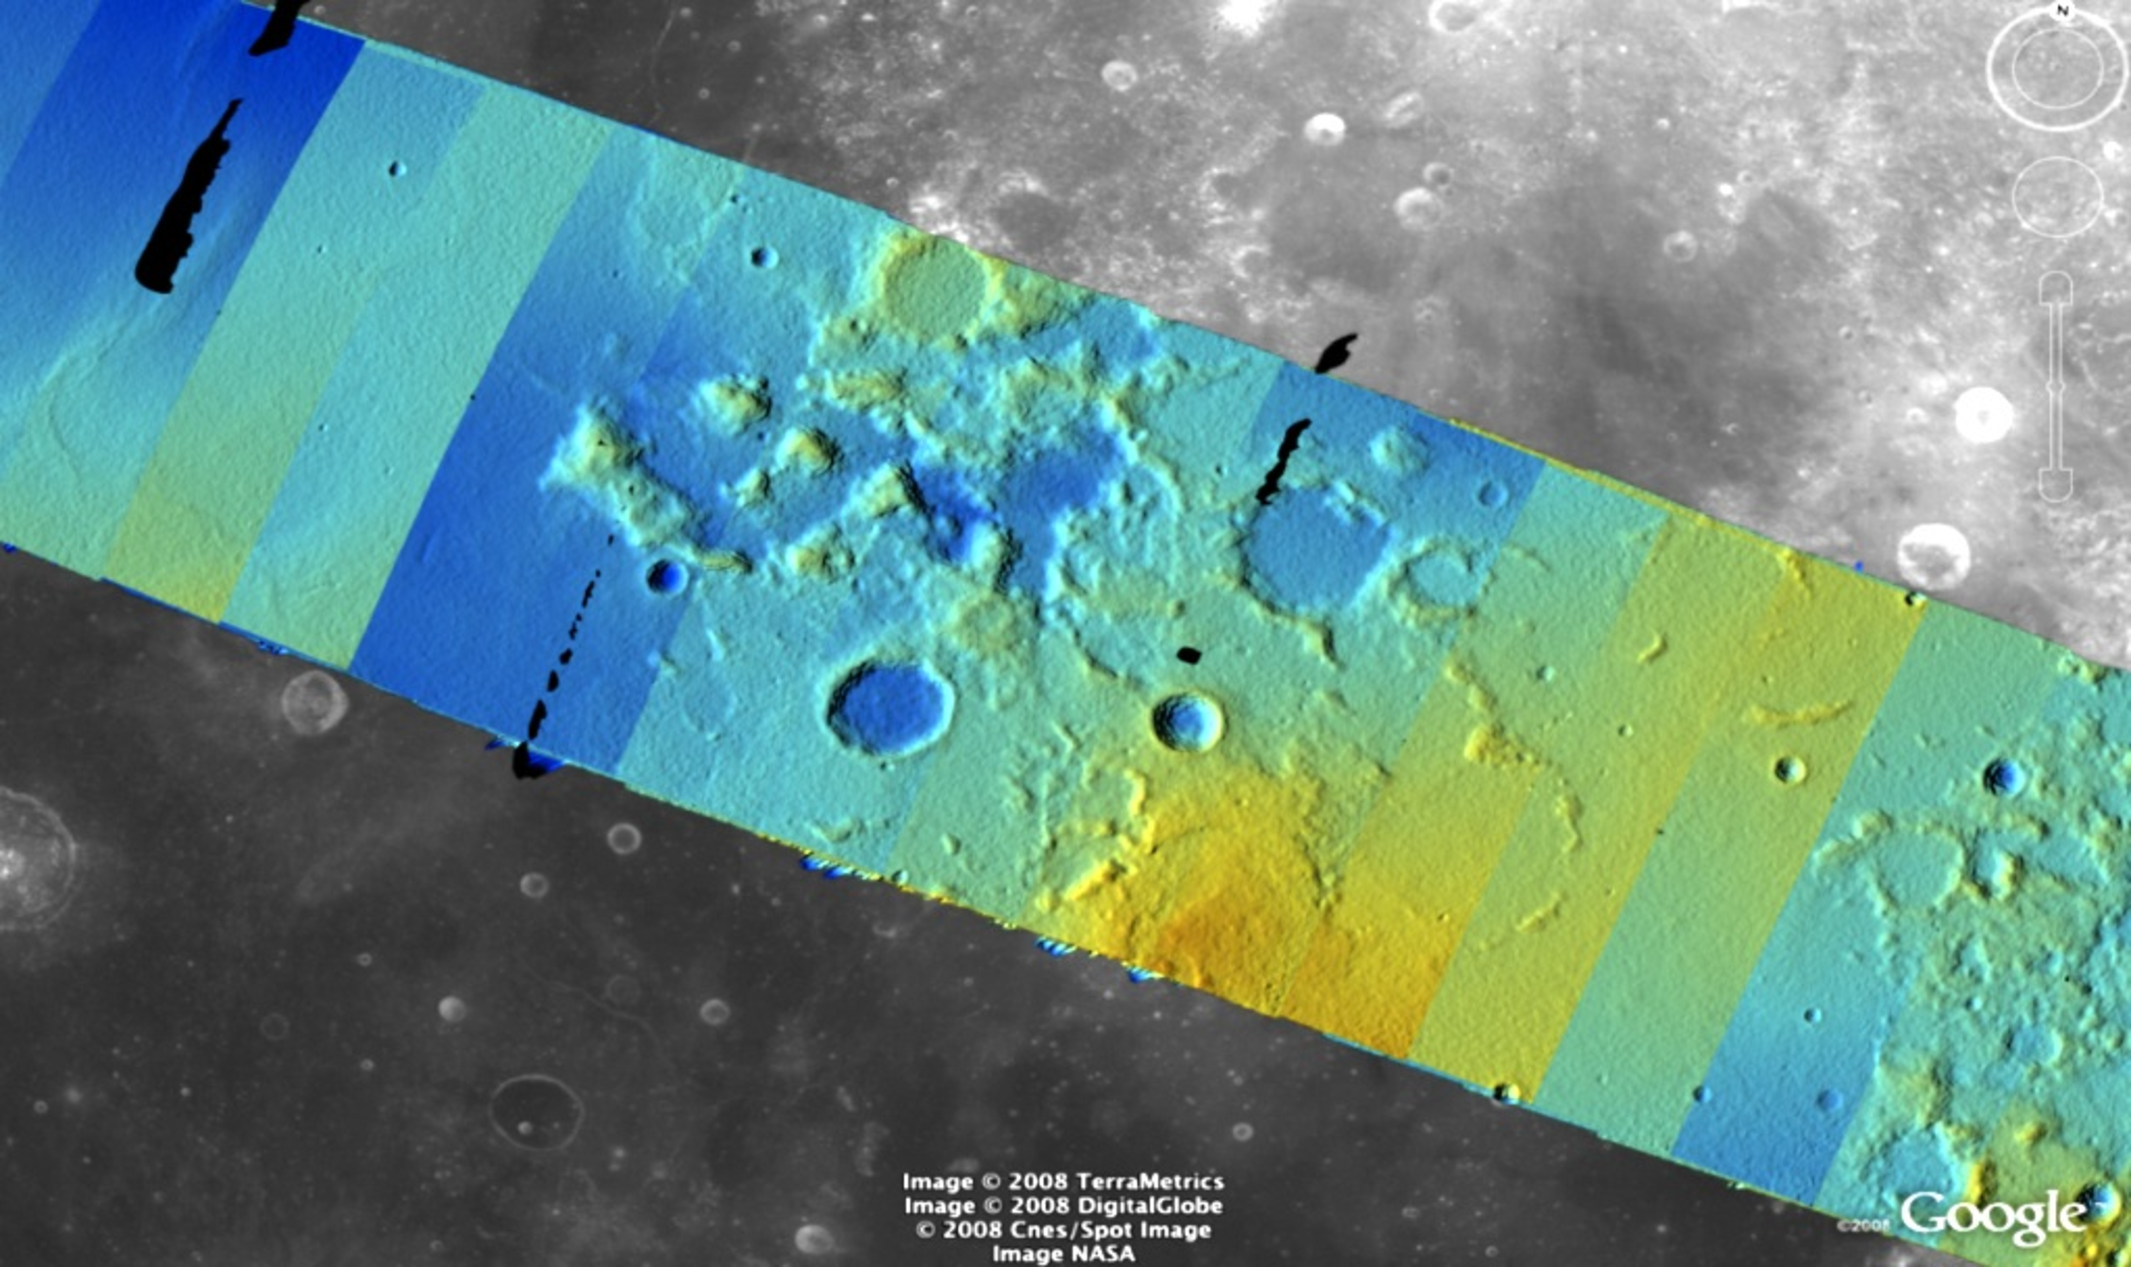
\includegraphics[width=8cm]{images/ba_orig}
  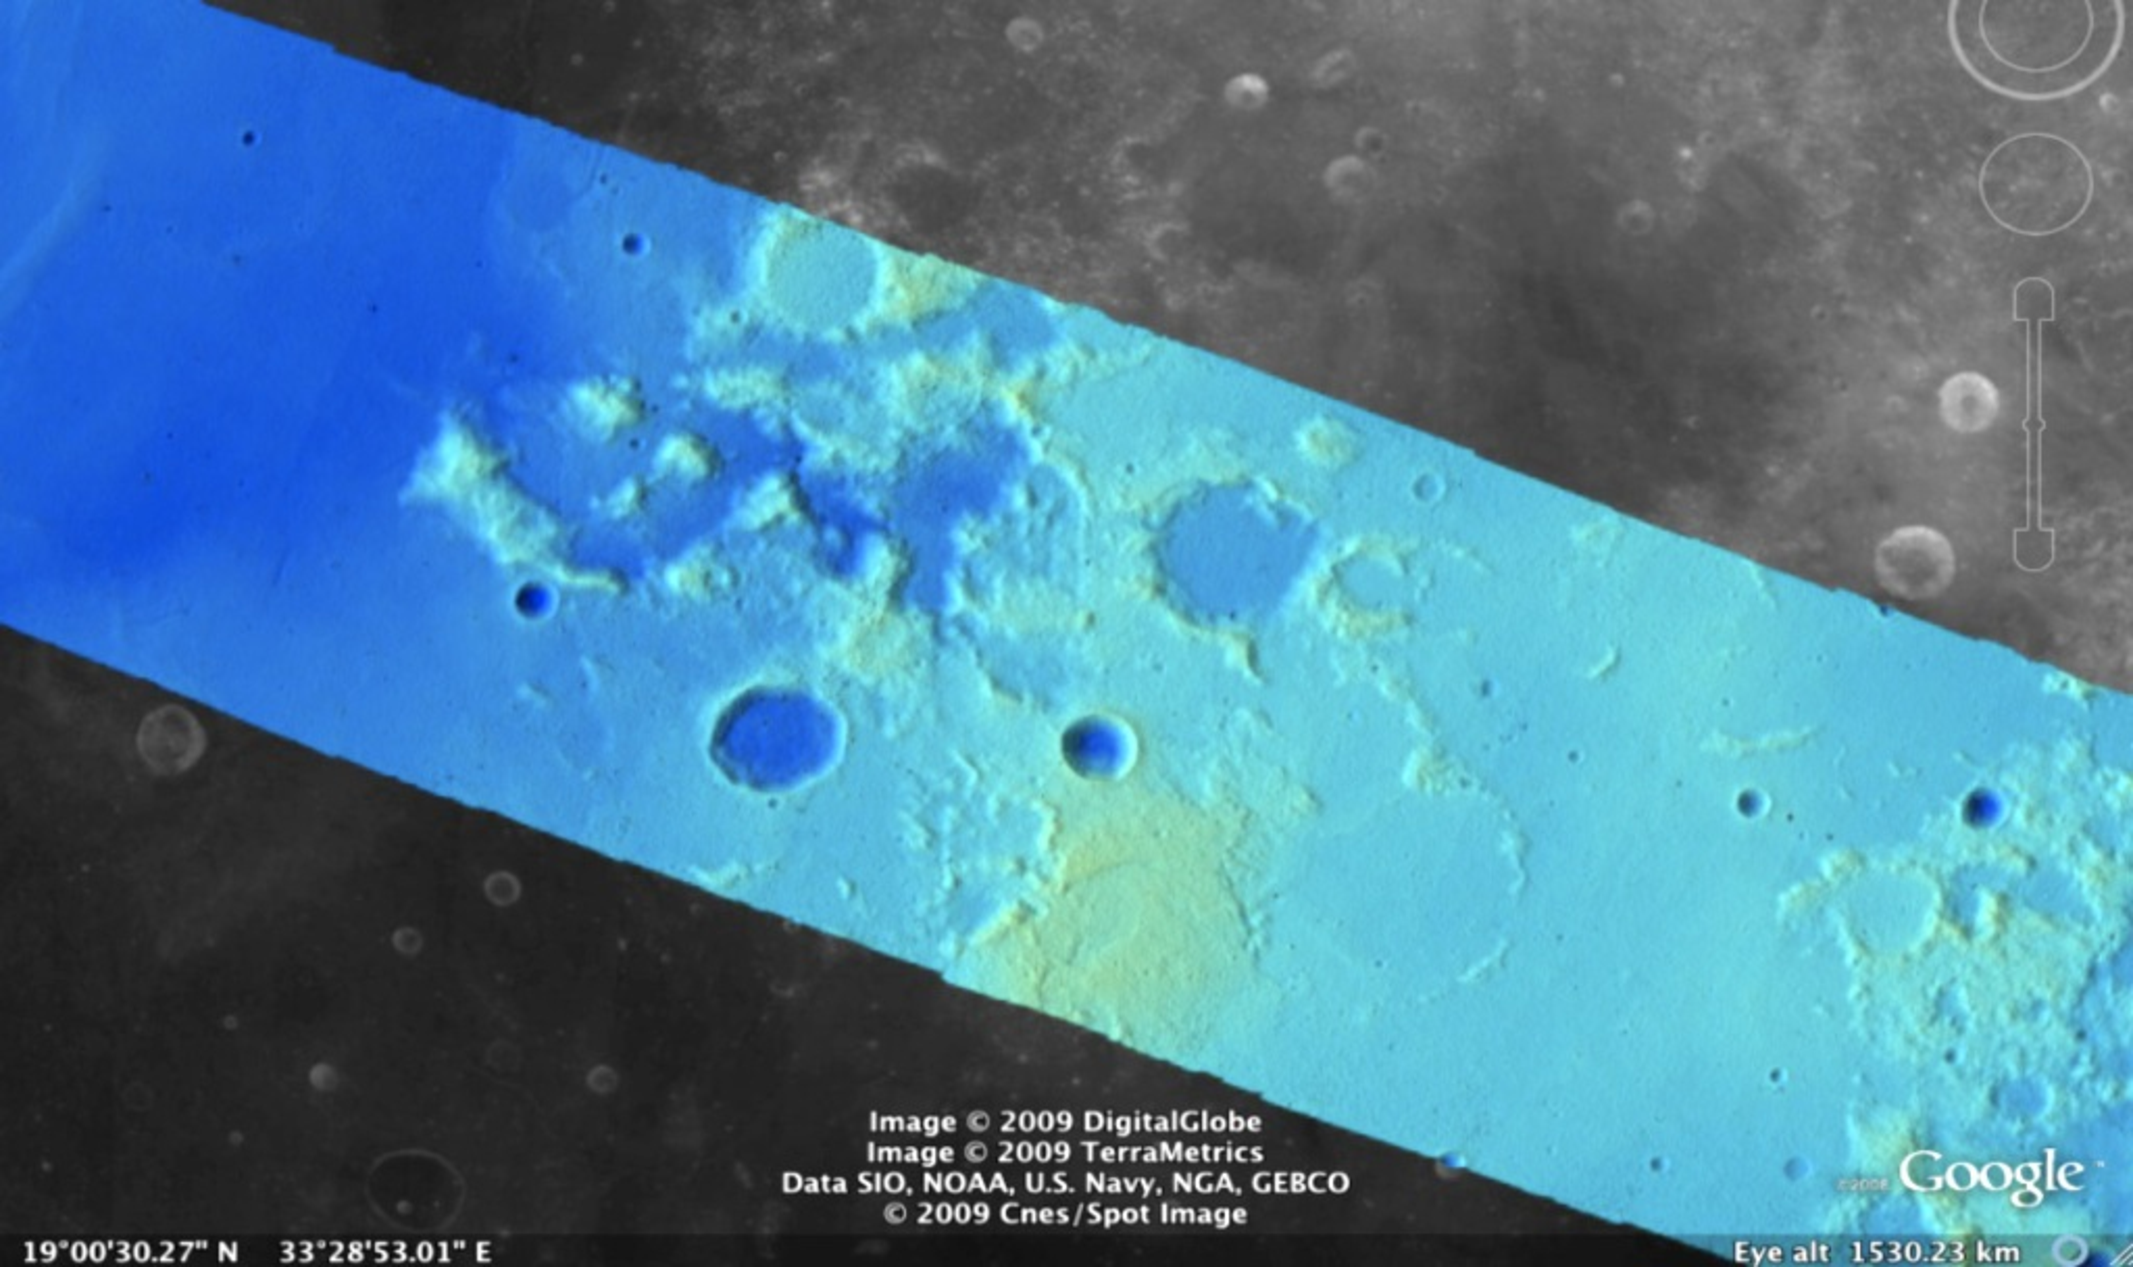
\includegraphics[width=8cm]{images/ba_adjusted}
  \caption{Bundle adjustment is illustrated here using a color-mapped,
    hill-shaded DEM mosaic from Apollo 15 Orbit 33 imagery. (a)
    Prior to bundle adjustment, large discontinuities can exist between
    overlapping DEMs made from different images. (b) After bundle
    adjustment, DEM alignment errors are minimized, and no longer visible.}
  \label{fig:bundle_adjustment}
\end{figure}

Bundle adjustment can also take advantage of ground control points
(GCPs), which are 3D locations of features that are known a
  priori (often by measuring them by hand in another existing
DEM). GCPs can improve the internal consistency of your DEM or align
your DEM to an existing data product. Finally, even though bundle
adjustment calculates the locations of the 3D objects it views, only
the final properties of the cameras are recorded for use by the Ames
Stereo Pipeline. Those properties can be loaded into the \texttt{stereo}
program which uses its own method for triangulating 3D feature
locations.

When using the Stereo Pipeline, bundle adjustment is an optional step
between the capture of images and the creation of DEMs.  The bundle
adjustment process described below should be completed prior to
running the \texttt{stereo} command.

\begin{center}
  \definecolor{lgray}{gray}{0.95}
  \fcolorbox{black}{lgray}{ \begin{minipage}{5.5in} Although Bundle
    Adjustment is not a required step for generating Digital Elevation
    Models, it is {\em highly recommended} for users who plan to
    create DEMs for scientific analysis and publication.
    Incorporating bundle adjustment into the stereo work flow not only
    results in DEMs that are more internally consistent, it is also
    the correct way to co-register your DEMs with other existing data
    sets and geodetic control networks.
\end{minipage}}
\end{center}


\subsection{A deeper understanding}

In bundle adjustment the position and orientation of each camera station are
determined jointly with the 3D position of a set of image tie-points
points chosen in the overlapping regions between images.
Tie-points are automatically extracted using the SURF robust feature
extraction algorithm \citep{surf08}.  Outliers are rejected using
the RANSAC method and trimmed to 1000 matches that are spread evenly
across the images.

\begin{figure}[b!]
  \begin{center}
  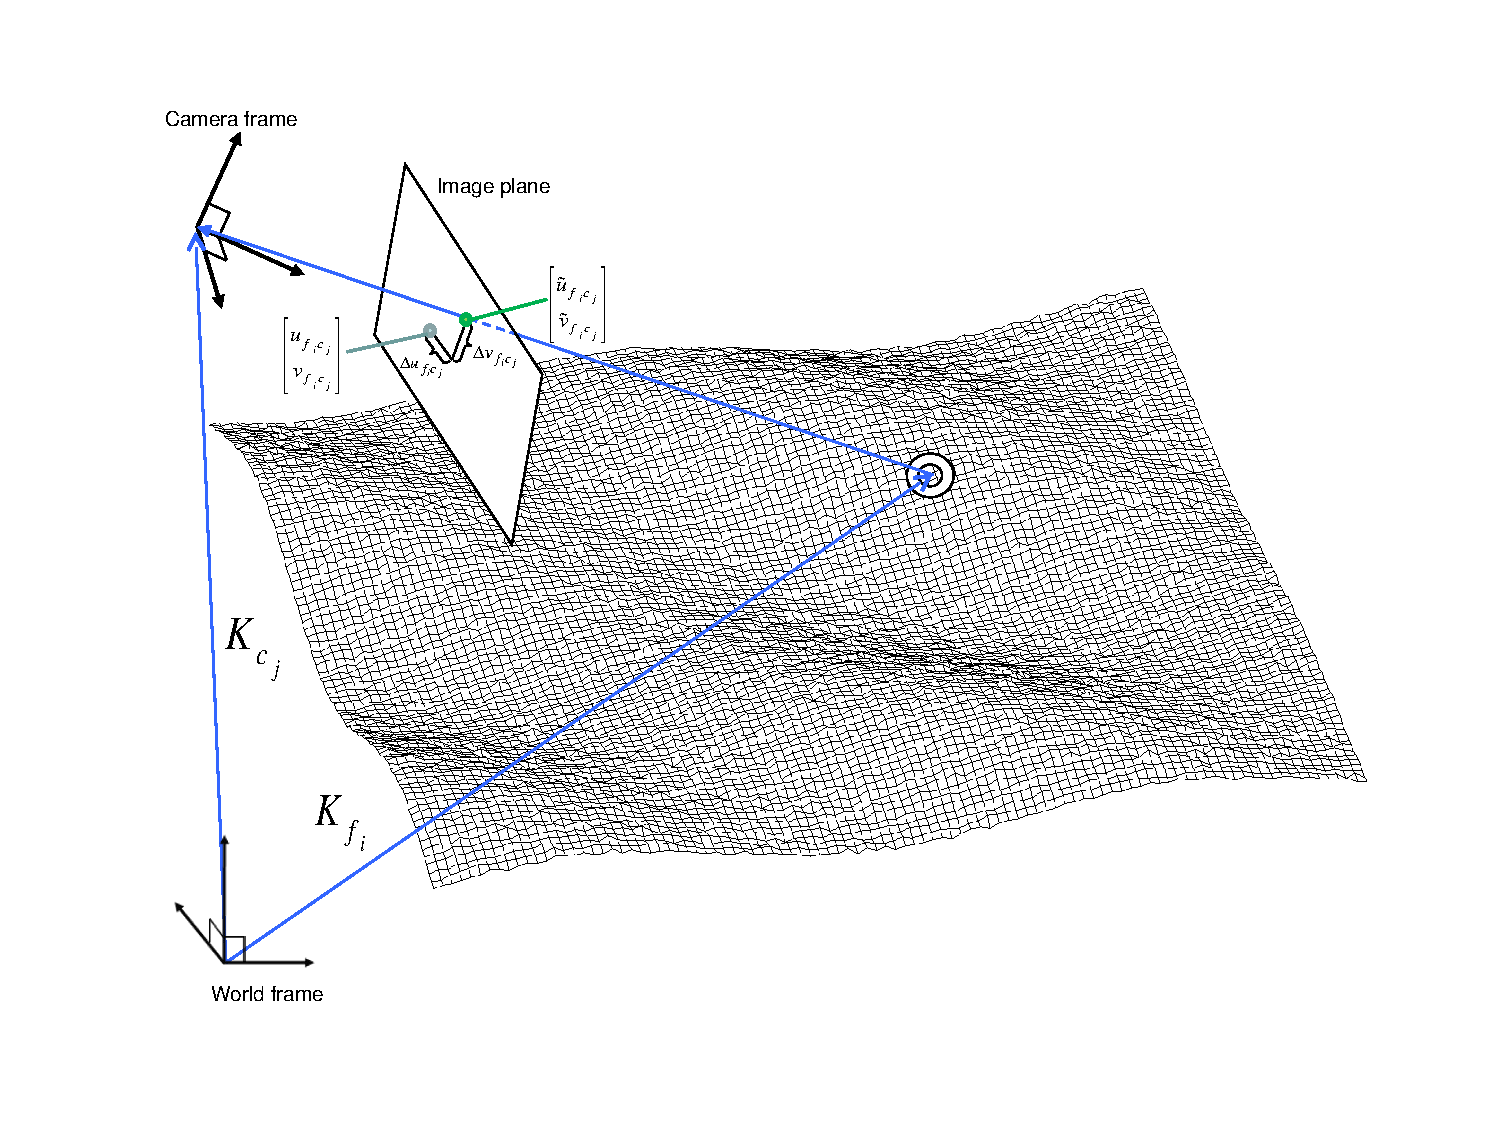
\includegraphics[trim=20mm 20mm 20mm 15mm,clip,width=6in]{images/ba_feature_observation.pdf}
  \end{center}
  \caption{ A feature observation in bundle adjustment \citep{moore09} }
  \label{fig:ba_feature}
\end{figure}

Our bundle adjustment approach follows the method described
in~\cite{triggs00} and determines the best camera
parameters that minimize the projection error given by ${\bf \epsilon}
= \sum_k\sum_j(I_k-I(C_j, X_k))^2$ where $I_k$ are feature locations
on the image plane, $C_j$ are the camera parameters, and $X_k$ are the
3D positions associated with features $I_k$. $I(C_j, X_k)$ is an image
formation model (i.e. forward projection) for a given camera and 3D
point.  The optimization of the cost function uses the
Levenberg-Marquardt algorithm (LMA). Speed is improved by using sparse
methods as described in \citet{hartley04}.

To eliminate the gauge freedom inherent in this problem, we add two
additional error metrics to this cost function to constrain the position
and scale of the overall solution. First, ${\bf \epsilon} =
\sum_j(C_j^{initial}-C_j)^2$ constrains camera parameters to stay
relatively close to their initial values.  Second, a small handful of
3D ground control points are chosen by hand and added to the
error metric as ${\bf \epsilon} = \sum_k(X_k^{gcp}-X_k)^2$ to
constrain these points to known locations in the planetary coordinate
frame.  In the cost functions discussed above, errors are weighted by
the inverse covariance of the measurement that gave rise to the
constraint.

Like other iterative optimization methods, there are several
conditions that will cause bundle adjustment to terminate.  When
updates to parameters become insignificantly small or when the error,
${\bf \epsilon}$, becomes insignificantly small, then the algorithm
has converged and the result is most likely as good as it will get.
However, the algorithm will also terminate when the number of
iterations becomes too large, in which case bundle adjustment may or
may not have finished refining the parameters of the cameras.  

\section{ISIS Adjust}

The \texttt{isis\_adjust} program is designed to perform bundle
adjustment on images supported by USGS's ISIS 3 software package.
The \texttt{isis\_adjust} program is special in that it does not
discriminate based on camera type. It can perform bundle adjustment
on line-scan imagers (e.g. MOC, LROC-NAC, HiRISE, and CTX) just
as well as it can on traditional frame cameras (e.g. Apollo
Metric Camera).  Theoretically it should also work fine with
push-frame imagers (e.g. THEMIS-VIS, LROC-WAC), though this is untested.

The \texttt{isis\_adjust} program works by first converting all
pixel measurements in an image to measurements defined on the ideal
focal plane using millimeters and the ephemeris time (ET). The ET
is the absolute second at which that pixel measurement was recorded
on the camera.  For a frame camera, all of the pixels are captured
at the same time so the ET will be identical for all measurements
on the image.  For pushbroom, pushframe, or other cameras which
build up their `image' over time, different parts of the image will
have different ET values.  For example, on a MOC image between the
first and last line about 5 seconds of ET will have elapsed.


When \texttt{isis\_adjust} calculates the partial derivatives of the
forward projection of a point, it uses an ideal pinhole camera model.
The properties of this model are defined as properties of the subject
camera at the specified ET for the current measure plus the
correction function, $f(t)$, that \texttt{isis\_adjust} is solving
for.  Many forms of $f(t)$ could be used; the only limit is the
number parameters in the equations. Some initial work hints that
anything greater than a second order polynomial becomes an ill-posed
problem, but we hope to investigate this further in the future.

\begin{center}
  \definecolor{lgray}{gray}{0.95}
  \fcolorbox{black}{lgray}{ \begin{minipage}{5.5in}

      Currently \texttt{isis\_adjust} lacks a proper way to support
      arbitrarily defined correction functions, $f(t)$. For the time
      being, \texttt{isis\_adjust} has been hard-coded to perform only
      six degrees of freedom, time independent corrections (i.e. a
      single position and orientation correction that applies to the
      entire image).  We hope to support more exotic corrections, such
      as cubic spline adjustments for pushbroom images, in a future
      release. (03/11/09)
\end{minipage}}
\end{center}

\subsection{Options}

The following is a listing and explanation of the options
that can be given to \texttt{isis\_adjust} on the command line.

\begin{description}

\item[--cnet, -c \textnormal{\small{(control network file)}}] \hfill \\
  \emph{Optional.} This option will force {\tt isis\_adjust} to
  use a pre-built built control network. This control network can
  either be in the USGS ISIS ``cnet'' format or in the binary Vision
  Workbench format. 

  If no control network is supplied using this option, {\tt
    isis\_adjust} will look for match files in the current working
  directory with base filenames that match the input images.  The
  \texttt{isis\_adjust} program will then create its own control
  network file and save it as \texttt{isis\_adjust.cnet}.

\item[--lambda, -l \textnormal{\small{(= \emph{float})}}] \hfill \\
  \emph{Optional.} This sets the starting value for $\lambda$: the
  parameter in the Levenberg Marquardt (LMA) optimization algorithm
  that selects between Gauss-Newton optimization and gradient
  descent. This parameter evolves over time on its own, but this
  argument can be used to override its initial value. \emph{This is an
  advanced setting, not recommended for normal use.}

\item[--position-sigma \textnormal{\small{(default = 100)}}] \hfill \\
  Sets the sigma (or uncertainty) of the spacecraft position in
  units of meters.

\item[--pose-sigma \textnormal{\small{(default = 0.1)}}] \hfill \\
  Sets the sigma (or uncertainty) of the spacecraft pose in units
  of radians.

\item[--gcp-scalar \textnormal{\small{(default = 1)}}] \hfill \\
  Sets the multiplier that is used to adjust the sigma
  (or uncertainty) of the ground control points. The sigmas of ground
  control points are defined in the GCP data file, so this
  option is useful when debugging for universally scaling GCP sigmas up
  or down.

\item[--cost-function \textnormal{\small{(default=L2)}}] \hfill \\
  Sets the cost function used for bundle adjustment. Default is L2
  which is the normal squared error. The other options are
  PseudoHuber, Huber, L1, and Cauchy. These other options are robust
  cost functions that deal better with non-ideal data that has
  outliers.

\item[--robust-threshold \textnormal{\small{(default=10)}}] \hfill \\
  Sets the robust threshold; an additional parameter specifically for
  the PseudoHuber, Huber, and Cauchy cost functions.

\item[--run-match, -m] \hfill \\
  \emph{Optional.} If cached tie-point \texttt{*.match} files don't
  already exist, create them from available \texttt{*.vwip} files using a
  call to \texttt{ipmatch}.

\item[--match-debug-images, -d] \hfill \\
  \emph{Optional.} If the {\tt --run-match} option is being used, this
  option creates useful debugging images that show tie-point matches
  between the input images.

\item[--min-matches \textnormal{\small{(default = 5)}}] \hfill \\
  Set the minimum number of tie-points that are required between a
  pair of images for them to be included in the control network. This
  option is useful for eliminating tie-points from image pairs that
  have only a handful of poor or erroneous matches.

\item[--max-iterations \textnormal{\small{(default = 25)}}] \hfill \\
  Sets the maximum number of iterations for bundle adjustment. The
  number of required iterations will vary by problem size, so this
  parameter allows the user to decide how much time they're willing
  to dedicate to the correction of the data.  We have found that 20
  iterations suffices for small problems with 10 or fewer images, and
  tens or hundreds of iterations may be required for problems with
  hundreds or thousands of images.

\item[--report-level, -r \textnormal{\small{(default = 10)}}] \hfill \\
  Sets the report level for the final bundle adjustment report.  This
  report is saved as \texttt{isis\_adjust.report}. Report levels are
  defined in the \texttt{BundleAdjustReport.h} header file in the Vision
  Workbench camera module.

\item[--nonsparse, -n] \hfill \\
  \emph{Optional.} \texttt{isis\_adjust} normally uses a sparse
  implementation of the Levenberg Marquardt algorithm (LMA) that makes
  very efficient use of memory, even for large problems.  This option
  will cause the program to use a non-sparse version of LMA for
  debugging purposes.  This will run significantly slower and is
  only really designed to be used for debugging.

\item[--write-isis-cnet-also] \hfill \\

  \emph{Optional.} Write an ISIS PVL style control network file in
  \texttt{isis\_adjust.net}. The output file is very large compared to
  the binary output, \texttt{isis\_adjust.cnet}, but is human readable
  and compatible with the ISIS3 \texttt{qnet} tool.

\end{description}


\section{Visualizing Bundle Adjustment with BundleVis}

The \texttt{bundlevis} program is used to visualize the process of
bundle adjustment. It will show an animated, fully interactive 3D
scene containing all the 3D points and cameras across all iterations
of bundle adjustment.  This tool is used to quickly determine if
bundle adjustment was successful.  If something does go wrong,
\texttt{bundlevis} can be a powerful debugging tool for identifying
the problem.

\begin{figure}[t!]
  \begin{center}
  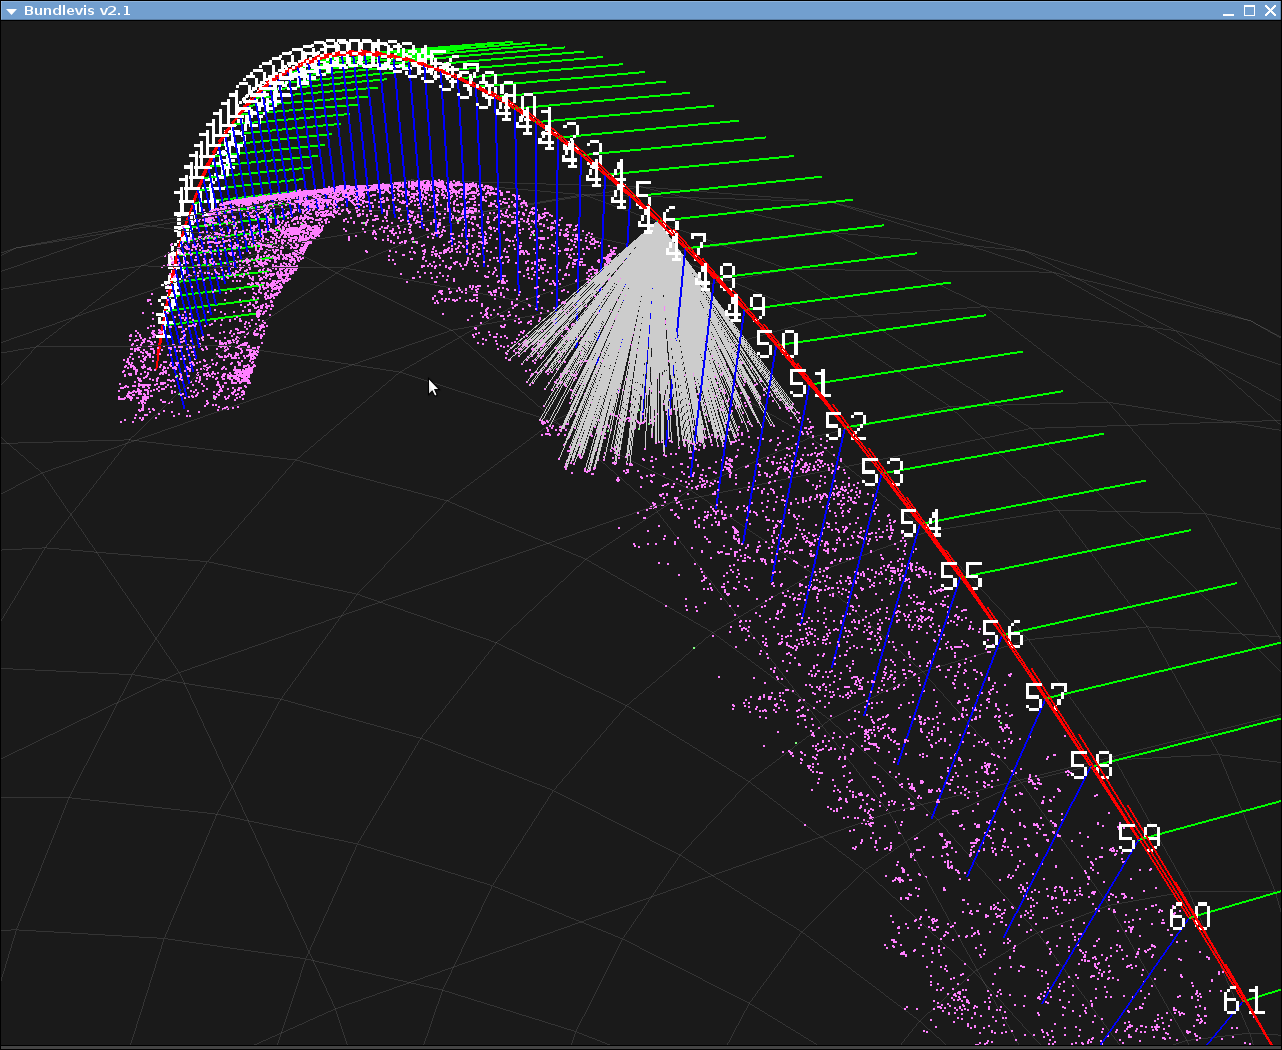
\includegraphics[width=5in]{images/bundlevis_apollo.png}
  \end{center}
  \caption{ A screenshot of \texttt{bundlevis} visualizing the bundle
    adjustment of imagery from the Apollo 15 Metric Camera (orbit
    33). }
  \label{fig:bundlevis}
\end{figure}

Once \texttt{bundlevis} has loaded the data from a bundle adjustment run,
the user can click on and inspect the position of 3D points that are
in purple and play back the iterations using the keyboard. Double
clicking on a camera will cause lines to be drawn to each point viewed
by the camera. Clicking on a 3D point causes lines to be drawn to all
cameras that view the point.

Failure of bundle adjustment looks different in every case, but there
are two failure modes to be especially on the look out for. First is
segmentation; where tie points will split into two or more distinct
groups, producing cliffs between or clumps among points. This is
usually caused by insufficient matches between a
pair of images in your control network.  You may need to choose some
tie-points between these images by hand or add additional images that
overlap with the problem area.

The second common sign of a failure is a point cloud explosion or
implosion. This most often results from a high number of outlying,
bad tie-point measurements. These bad constraints can be removed by
hand or mitigated using one of the robust cost modes (e.g. by using
the \texttt{--cost-function} argument for \texttt{isis\_adjust}).

\subsection{Options}

The following is a listing and explanation of the options
that can be given to \texttt{bundlevis} from the command line.

\begin{description}

\item[--camera-iteration-file, -c \textnormal{\small{(bundlevis camera iteration file)}}] \hfill \\
  \emph{Optional.} Supply a camera iteration file that was produced by
       \texttt{isis\_adjust}.  \texttt{bundlevis} will only draw cameras
       if you supply a camera iteration file.

\item[--points-iteration-file, -p \textnormal{\small{(bundlevis point iteration file)}}] \hfill \\
  \emph{Optional.} Supply a point iteration file that was produced by
       \texttt{isis\_adjust}.  \texttt{bundlevis} will only draw 3D points
       if you supply a point iteration file.

\item[--control-network-file, -n \textnormal{\small{(Vision Workbench binary control network file)}}] \hfill \\
  \emph{Optional.} Supply a control network file that was produced by
       {\tt isis\_adjust}.  This allows {\tt bundlevis} to show the
       relationship between points and cameras when used in
       conjunction with \texttt{--camera-iteration-file} and
       \texttt{--points-iteration-file}.

\item[--additional-pnt-files \textnormal{\small{(bundlevis point iteration files)}}] \hfill \\
  \emph{Optional.} Supply additional points to be animated alongside
  the camera and 3D points.  The files given must be in the same
  format as a bundlevis point iteration file and have the same number
  of iterations.

\item[--fullscreen] \hfill \\
  \emph{Optional.} Displays \texttt{bundlevis} using the entire screen;
  otherwise the program loads in a window. \emph{The fullscreen option
    does not work correctly with dual screen systems.}

\item[--stereo] \hfill \\
  \emph{Optional.} Render the 3D scene in red/blue anaglyph mode.

\item[--show-moon] \hfill \\
  \emph{Optional.} Draws a wireframe sphere with a radius of 1737.3-km
  that represents the Moon.

\item[--show-mars] \hfill \\
  \emph{Optional.} Draws a wireframe sphere with a radius of 3397-km
  that represents Mars.

\item[--show-earth] \hfill \\
  \emph{Optional.} Draws a wireframe sphere that represents the Earth.

\end{description}

\subsection{Controls}

Once \texttt{bundlevis} is running, there are several controls that
can be used to interface with the program. There are the playback
controls, jump-to-frame controls, and the mouse.

\paragraph{Playback Controls}

Playback controls are similar to winamp; arranged on the keyboard like
the controls on a tape deck.

\newenvironment{myindentpar}[1]
               {\begin{list}{}
                   {\setlength{\leftmargin}{#1}}
                 \item[]
               }
               {\end{list}}

\begin{myindentpar}{3cm}
\begin{description}
  \item[Z] Step back one iteration
  \item[X] Play
  \item[C] Pause
  \item[V] Stop \emph{(which is the same as Pause except that
    bundlevis goes back to iteration 0)}
  \item[B] Step forward one iteration
\end{description}
\end{myindentpar}

\paragraph{Jump-to-Frame Controls}
Jump-to-Frame controls are the numbers \textbf{1-9} along the top of
the keyboard. Pressing \textbf{1} will display the very first
iteration. Pressing \textbf{9} will display the very last
iteration. Pressing \textbf{2} through \textbf{8} will display
iterations that are somewhere in between based on the value of the
number. Finally, pressing \textbf{0} will cause \texttt{bundlevis} to
display the points at their very last iteration with an additional
tail pointing back to the starting position of the points in the first
iteration.

\paragraph{Mouse}
The mouse is used to move around the model, and has the same controls
found in many 3D environments (e.g. \texttt{osgviewer}). Moving the
mouse with the \textbf{left mouse button} held down will cause the
model to rotate.  Moving with the \textbf{right mouse button} pressed
will zoom, and moving with the \textbf{middle mouse button} will
translate. Alternatively for systems where the mouse is
button-challenged, \textbf{option + mouse} is translation and
\textbf{command + mouse} is zoom. 

Double clicking with the mouse on a point or camera will allow the
user to query entities in the model.  A double click will cause the
point number and camera number to be printed to the terminal. The
number identifier for a given camera or point will also appear when
the viewer is zoomed in on that entity.

\section{Examples of Use}

\subsection{Processing Mars Orbital Camera}

What follows is an example of bundle adjustment using two Mars Orbital
Camera (MOC) images of the south Cydonia region. We use images
M10/00254 and R09/01059. These images are available from NASA's
Planetary Data System (be sure to download the IMQ or IMG format
files). For reference, the following ISIS commands are how to convert
the MOC images to ISIS cubes.

\begin{verbatim}
        mocproc from= m1000254.im? to= m1000254.cub Mapping= NO
        mocproc from= r0901059.im? to= r0901059.cub Mapping= NO
\end{verbatim}

At this point, we need to automatically generate tie-points between
these two images.  This can be done using the \texttt{ipfind} and
\texttt{ipmatch} utilities.  These tools do not (currently) work
with photometrically calibrated images, so we must first convert
these images to a standard format using the ISIS program \texttt{isis2std}:

\begin{verbatim}
        isis2std from= m1000254.cub to= m1000254.png format= PNG
        isis2std from= r0901059.cub to= r0901059.png format= PNG
\end{verbatim}

Here is how to process those newly created PNG files for tie-points
using the tools available in Vision Workbench.

\begin{verbatim}
        ipfind  m1000254.png r0901059.png
        ipmatch m1000254.png r0901059.png -d -r homography
\end{verbatim}

\definecolor{lgray}{gray}{0.95}
\begin{center}
\fcolorbox{black}{lgray}{ \begin{minipage}{5.5in} 

    We are aware that the tie-point tools available in Vision
    Workbench do not always produce enough matches for bundle
    adjustment. An alternative that we have found works quite well is
    to use an outside method such as SURF \citep{surf08}. We have
    included a small example program that converts SURF output to a
    Vision Workbench style match file.  \\ \\ For this example it is
    okay to use the results from \texttt{ipfind} and
    \texttt{ipmatch}. Expect to find approximately 46 matched
    points. Your results will be slightly different due to the random
    nature of RANSAC.

\end{minipage}}
\end{center}

Finally it is time to start bundle adjustment. There are many options
that can be used at this stage.  We have chosen those required to
create visualization data for \texttt{bundlevis}.  We have also set
the maximum iterations to 100 and chosen the option to create a
detailed report file of \texttt{isis\_adjust}'s results.

\begin{verbatim}
        isis_adjust *.cub -s --max 100 -r 50
\end{verbatim}

This command will produce considerable debugging output and will
place many output files in the current working directory. Don't
panic--this is perfectly normal! If you look through the output in
the terminal or alternatively in the output report file,
\texttt{isis\_adjust.report}, you'll see that the problem converged
in 35 iterations (again, your results may vary slightly).  The error
is improved only slightly, which can be attributed to Mars Global
Surveyor's relative positioning between images being pretty good
for this case.

Visualizing all the data that was exported for \texttt{bundlevis} can
be carried out as follows:

\begin{verbatim}
        bundlevis -p iterPointsParam.txt -c iterCameraParam.txt 
                  -n isis_adjust.cnet
\end{verbatim}

Press escape to exit out of \texttt{bundlevis} when finished.  You may
also want to try viewing the data with a wireframe of Mars to give
some perspective. Note, you will have to zoom in very far since the
size of a MOC frame is quite small relative to the size of Mars!

\begin{verbatim}
        bundlevis -p iterPointsParam.txt -c iterCameraParam.txt
                  -n isis_adjust.cnet --show-mars
\end{verbatim}

Producing a DEM using the newly created corrections is the same as
covered in Chapter 3, with one small difference: \texttt{stereo} needs
to know of the existence of the correction files,
\texttt{m1000254.isis\_adjust} and \texttt{r0901059.isis\_adjust}:

\begin{verbatim}
        stereo m1000254.cub r0901059.cub m1000254.isis_adjust
               r0901059.isis_adjust MOC_RESULTS/M1000254_R0901059
\end{verbatim}

Note the two new arguments (\texttt{*.isis\_adjust}) to \texttt{stereo}
that provide it with the necessary corrections.

\subsection{Processing with Ground Control Points}

Just as \texttt{isis\_adjust} will automatically look for match files
in the current working directory, it will also search for ground
control points. Ground control point files are written with the
extension \texttt{.gcp} and are expected to have the same name as the
image file that they are describing.

Below is an example of a ground control point file that was created to
control an Apollo Metric Camera image (AS15-M-1125) from Apollo 15's
Orbit 33.

\begin{verbatim}
   3305     3811    17.081049  20.173588  1734697.6    100   100   100
   1676.37  926.12  15.638650  24.560510  1734771.35   100   100   100
   3646.08  631.37  18.663032  24.358845  1734745.22   100   100   100
   1206.38  2995.9  14.306318  21.909843  1734746.16   100   100   100
   2872     2154    16.983669  22.560025  1734726.48   100   100   100
\end{verbatim}

First it's important to note that these numbers are not spaced with
actual spaces, but instead there is a tab character between each
column of numbers. Here is what the columns mean:

\begin{myindentpar}{2cm}
\begin{description}
  \item[Column 1:] Sample Number or X location in pixels
  \item[Column 2:] Line Number or Y location in pixels
  \item[Column 3:] Longitude in degrees 
  \item[Column 4:] Latitude in degrees
  \item[Column 5:] Radius in meters
  \item[Column 6-8:] Sigma (or uncertainty) in meters in the X, Y,
    and Z directions respectively.
\end{description}
\end{myindentpar}

If multiple cameras see the same ground control point, then in each
GCP file at the line containing the shared measurement you will
need to make sure that the GCP has the exact same recorded longitude,
latitude, and radius. The \texttt{isis\_adjust} program will notice
this and will register a single GCP with multiple observations in
the control network.

\subsection{Sharing Data with ISIS3's Qnet}

ISIS contains a program called \texttt{qnet} whose purpose is to
create and edit ISIS style control network files. To share a control
network with \texttt{qnet}, you will need to save our control network
in the ISIS format. If bundle adjustment has already been performed
once and if we want to simply convert the control network for use in
\texttt{qnet}, you can use this command to save an ISIS style control:
network:

\begin{verbatim}
        isis_adjust -c isis_adjust.cnet --write-isis-cnet-also *.cub
\end{verbatim}

Otherwise if this is the first time performing bundle adjustment and a
control network does not already exist, use:

\begin{verbatim}
        isis_adjust --write-isis-cnet-also *.cub
\end{verbatim}

There should now be an \verb=isis_adjust.net= file in the project's
directory. It will be quite a bit larger than the other control
network file since it is stored as ASCII text, but it can be read and
edited with a text editor. Before starting \texttt{qnet}, there is one
additional preparation that must be performed. ISIS's \texttt{qnet} requires
a text file listing of all the cubes used by the control
network. Here's how to create one:

\begin{verbatim}
        ls *.cub > list_of_cubes.lis
\end{verbatim}

Now, start up \texttt{qnet} without any command line arguments. Click
File$\rightarrow$Open. It will first ask for the list of cubes. Refer
it to the newly created \texttt{list\_of\_cubes.lis}. Next it will ask for
the control network. Give it \texttt{isis\_adjust.net}.

\begin{center}
\fcolorbox{black}{lgray}{ \begin{minipage}{5.5in}

    At this time \texttt{qnet} does not work with the Apollo Metric
    Camera's cube files. When loading the text file listing of cubes
    it will issue error about invalid serial numbers for the listed
    cube files. (03/11/09)

\end{minipage}}
\end{center}

When finished, save the new control network file. Here's how to use
the new control network in \texttt{isis\_adjust}:

\begin{verbatim}
        isis_adjust -c the_new_control_network.net *.cub
\end{verbatim}

% \begin{thebibliography}{1}
% 
% \bibitem{hartley04} Hartley, R.I. and Zisserman, A. ``Multiple View Geometry in Computer Vision,''
%   Cambridge University Press. 2004. pp 597-627.
% \bibitem{moore09} Moore, Wright, Schinstock, and Lewis. ``Comparison of Bundle Adjustment Formulations,''
%   presented at ASPRS Annual Conf., Baltimore, Maryland, 2009.
% \bibitem{triggs00} Triggs, McLauchlan, Hartley, and Fitzgibbon. ``Bundle Adjustment - A Modern Synthesis,''
%   Lecture Notes in Computer Science. Vol. 1883, 298. January 2000
% \bibitem{surf09} Bay, Gool, and Tuytelaars. (2009, Mar.). ``SURF: Speeded Up Robust Features'' [Online]. Available: \verb!http://www.vision.ee.ethz.ch/~surf/download.html!
% 
% \end{thebibliography}
